The discrete nonlinear Schr\"dinger equation (DNLS)
\[
i \dot{u}_n + d(u_{n+1} - 2 u_n + u_{n-1}) + |u_n|^2 u_n
\]
is an analogue to the nonlinear Schr{\"o}dinger equation on the integer lattice,
and has applications to nonlinear optics and condensed matter physics \cite{Kevrekidis2009}. The parameter $d$ quantifies the coupling between adjacent lattice nodes. For all values of $d$, DNLS has a stable, primary pulse solution (\cref{fig:DNLS2p}, left). Provided that the individual peaks are separated by a sufficiently large number of lattice points, I use Lin's method to prove that multi-pulse solutions exist as long as the following geometric constraint is satisfied: neighboring peaks must either be out-of-phase or in-phase \cite[Theorem 4]{Parker2020}. Furthermore, I prove that this geometry determines the stability of multi-pulses \cite[Theorem 5]{Parker2020}. For double pulses, the in-phase double pulse is unstable, since there is eigenvalue with positive real part, and the out-of-phase double pulse is neutrally stable, since the entire spectrum lies on the imaginary axis (\cref{fig:DNLS2p}, center and right). The only neutrally stable multi-pulses are those in which every pair of neighboring peaks is out-of-phase. The proof of this result uses Lin's method to construct the eigenfunctions corresponding to the interaction eigenvalues. This reduces the spectral problem to finding the eigenvalues of a matrix.

\begin{figure}
    \centering
    \begin{tabular}{ccc}
        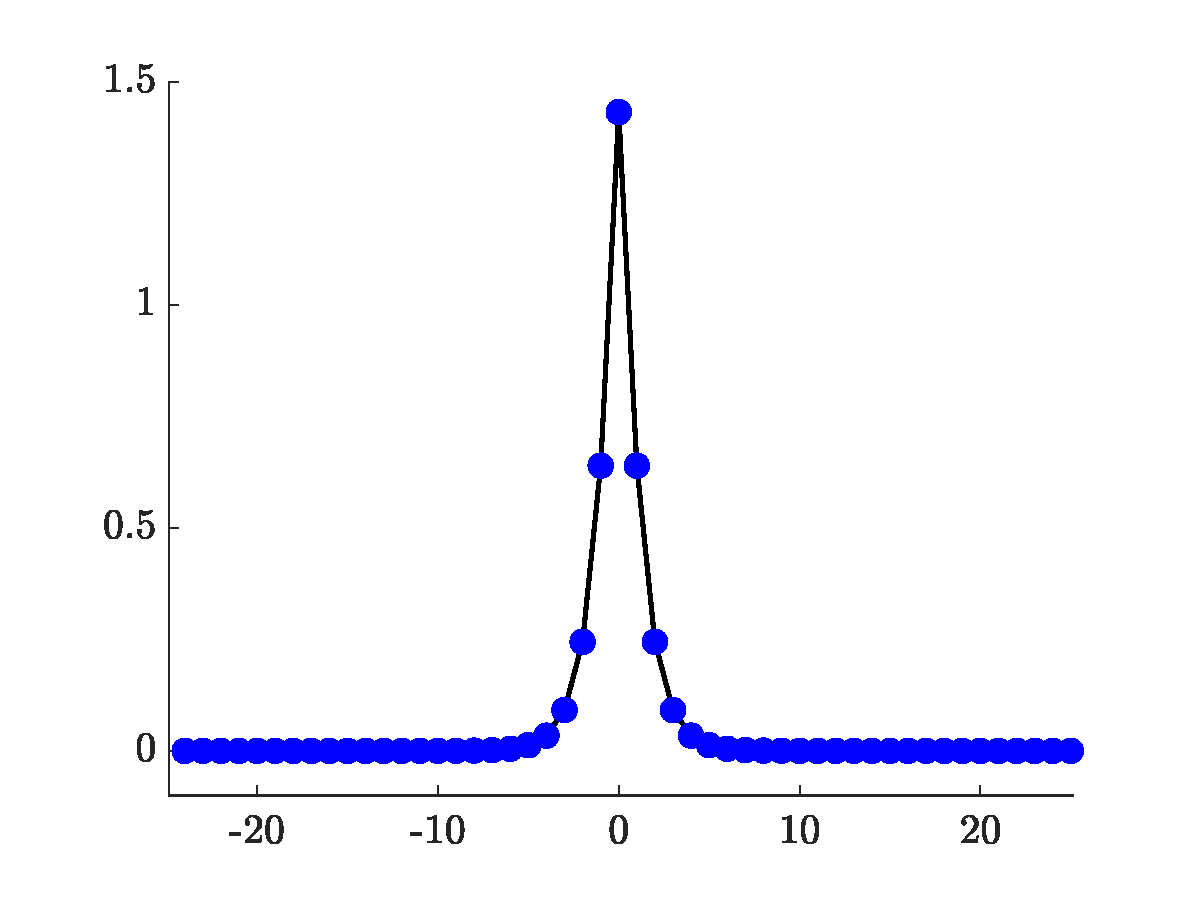
\includegraphics[width=5cm]{images/DNLSprimary.eps} &
        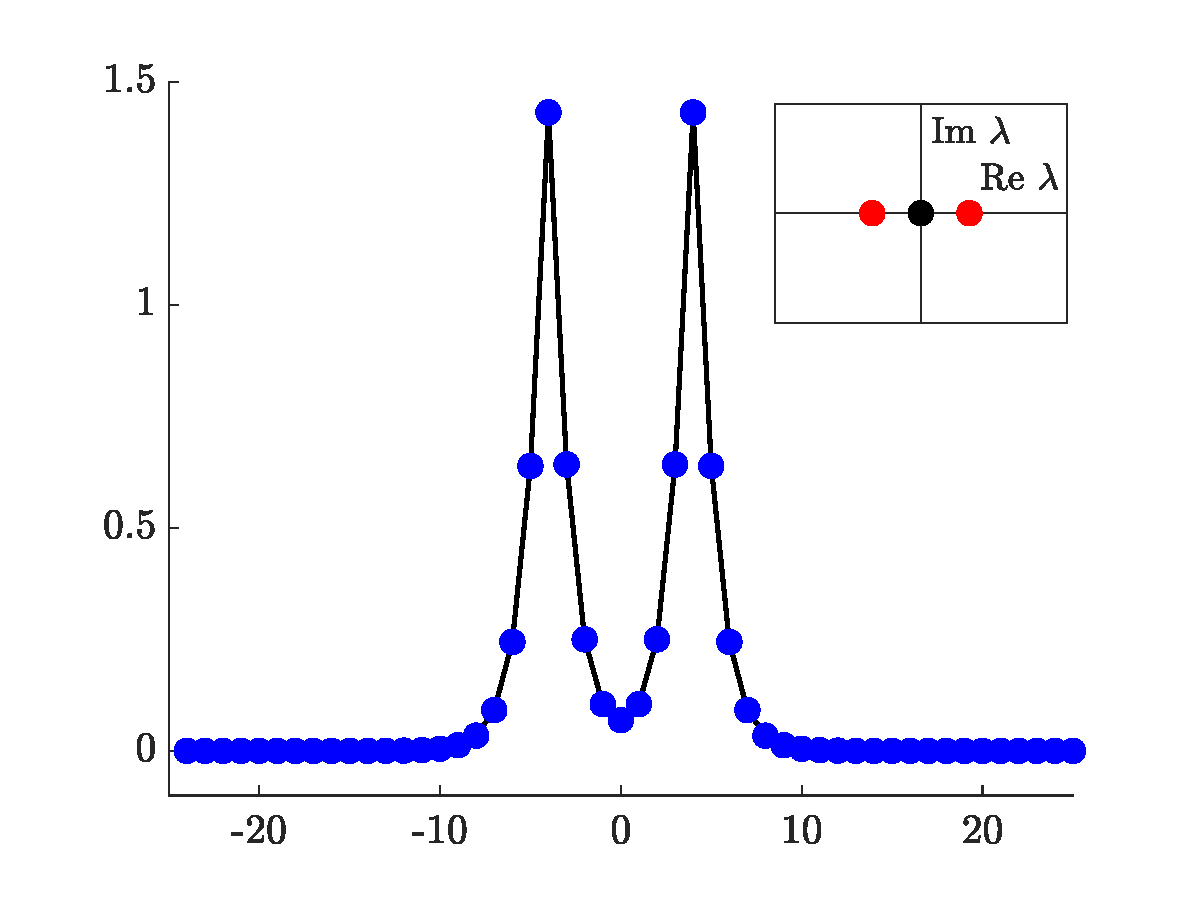
\includegraphics[width=5cm]{images/DNLSunstable2p.eps} &
        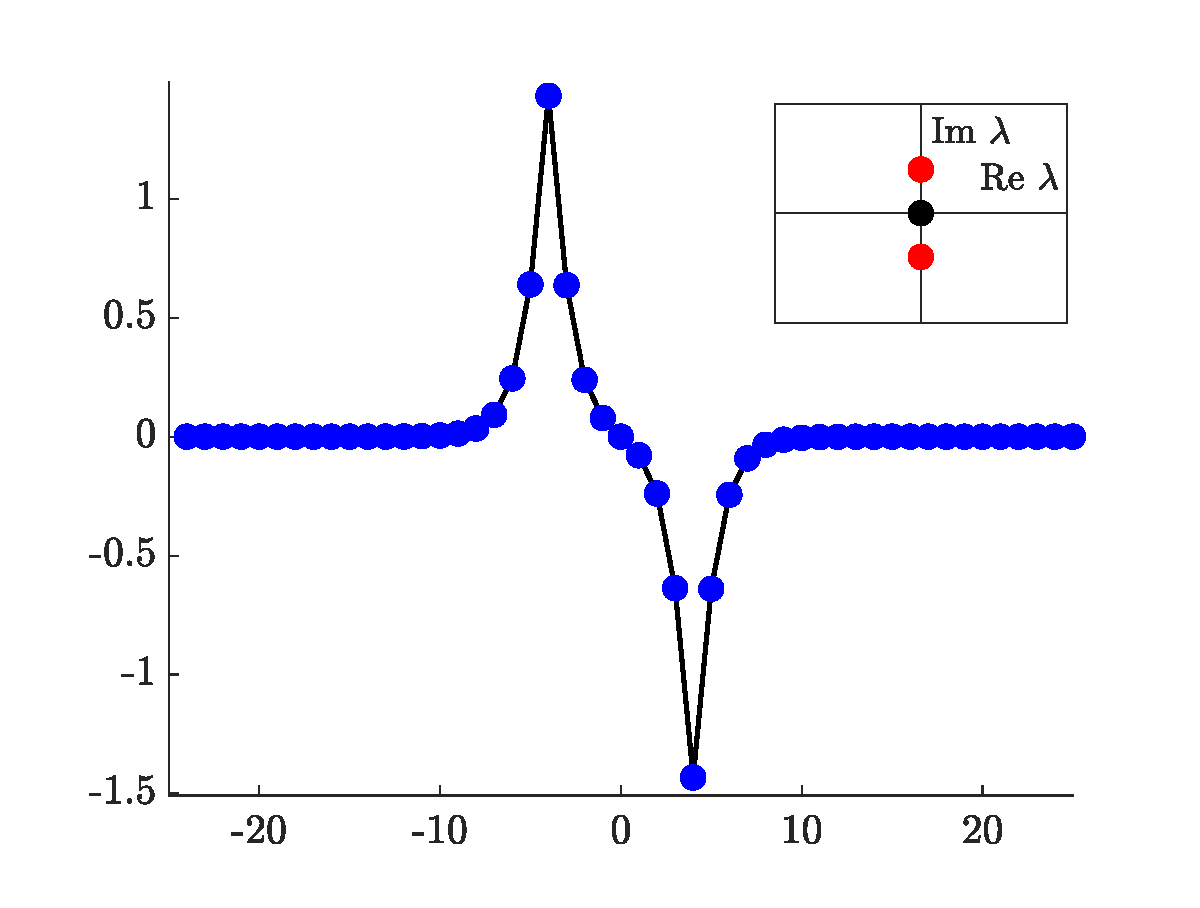
\includegraphics[width=5cm]{images/DNLSstable2p.eps} 
    \end{tabular}
    \caption{Primary pulse (left), out-of-phase double pulse (middle), and in-phase double pulse (right) solutions for DNLS. Interaction eigenvalue patterns for double pulses are shown in insets. Black dot is a kernel eigenvalue with algebraic multiplicity 2.}
    \label{fig:DNLS2p}
\end{figure}

Other discrete systems I have studied include multi-kinks \cite{ParkerSG} and multi-breathers \cite{Parker2022DKGbreathers} in the discrete Klein-Gordon equation. 
Future directions include extensions to models in which the coupling term involves longer range interactions, as well as models such as Fermi-Pasta-Ulam-Tsingou (FPUT) lattices in which the nonlinearity involves off-site terms. Another class of natural extensions is to look at higher dimensional lattices. In two dimensions, there are many possible regular lattice models, including square, triangular, and honeycomb, and these different geometries may exhibit qualitatively different behavior. 